% Propósito: separar las magnitudes de tres etapas de la generación sonora:
% señal eléctrica, desplazamiento del cono y perturbación acústica.
% Origen: cadena conceptual de la sección \ref{sec:u3-tono-puro}.
% Esquema funcional, no representa una respuesta medida ni presupone una
% relación cuantitativa entre amplitudes.
% Descripción accesible: tres bloques conectados. Una tensión eléctrica en
% volts excita un parlante; su cono se desplaza en metros; el movimiento genera
% desplazamiento de partícula en metros y presión acústica en pascales.
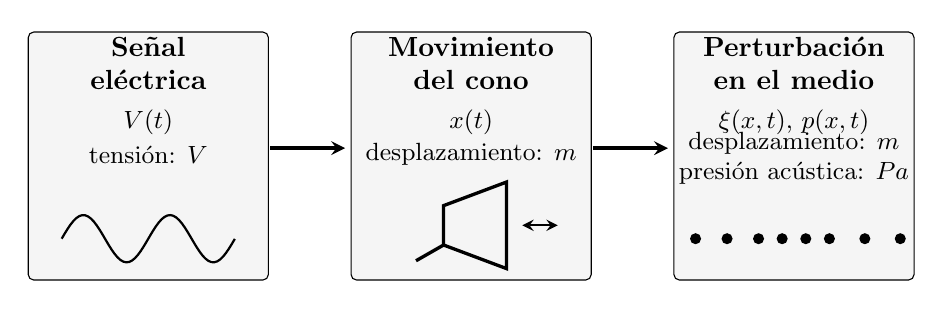
\begin{tikzpicture}[
    font=\small,
    >=stealth,
    etapa/.style={
        draw,
        rounded corners=2pt,
        minimum width=3.05cm,
        minimum height=3.15cm,
        align=center,
        fill=black!4
    }
]
    \node[etapa] (electrica) at (1.60,0) {};
    \node[etapa] (cono) at (5.70,0) {};
    \node[etapa] (medio) at (9.80,0) {};

    \node[font=\bfseries,align=center] at (1.60,1.18)
        {Señal\\eléctrica};
    \node at (1.60,0.43) {\(V(t)\)};
    \node at (1.60,0.02) {tensión: \(\text{V}\)};

    \node[font=\bfseries,align=center] at (5.70,1.18)
        {Movimiento\\del cono};
    \node at (5.70,0.43) {\(x(t)\)};
    \node at (5.70,0.02) {desplazamiento: \(\text{m}\)};

    \node[font=\bfseries,align=center] at (9.80,1.18)
        {Perturbación\\en el medio};
    \node at (9.80,0.43) {\(\xi(x,t)\), \(p(x,t)\)};
    \node[align=center] at (9.80,-0.03)
        {desplazamiento: \(\text{m}\)\\presión acústica: \(\text{Pa}\)};

    \draw[->,very thick] (3.15,0.10) -- (4.10,0.10);
    \draw[->,very thick] (7.25,0.10) -- (8.20,0.10);

    % Glifos conceptuales, sin escala.
    \draw[thick,samples=60,domain=0:1]
        plot ({0.50+2.20*\x},{-1.05+0.30*sin(720*\x)});
    \draw[very thick] (5.00,-1.33) -- (5.35,-1.13)
        -- (5.35,-0.63) -- (6.15,-0.33)
        -- (6.15,-1.43) -- (5.35,-1.13);
    \draw[<->,thick] (6.35,-0.88) -- (6.80,-0.88);
    \foreach \x in {8.55,8.95,9.35,9.65,9.95,10.25,10.70,11.15}{
        \fill (\x,-1.05) circle (2pt);
    }
\end{tikzpicture}
